\documentclass[12pt, twoside]{article}
% \documentclass[12pt, twoside]{article}
\usepackage[letterpaper, margin=1in, headsep=0.2in]{geometry}
\setlength{\headheight}{0.6in}
%\usepackage[english]{babel}
\usepackage[utf8]{inputenc}
\usepackage{microtype}
\usepackage{amsmath}
\usepackage{amssymb}
%\usepackage{amsfonts}
\usepackage[nomessages]{fp} %\FPeval{\var-name}{2*sin(pi/6)}
\usepackage{siunitx} %units in math. eg 20\milli\meter
\usepackage{yhmath} % for arcs, overparenth command
\usepackage{tikz} %graphics
\usetikzlibrary{quotes, angles, arrows, arrows.meta}
\usepackage{graphicx} %consider setting \graphicspath{{images/}}
\usepackage{parskip} %no paragraph indent
\usepackage{enumitem}
\usepackage{multicol}
\usepackage{venndiagram}

\usepackage{fancyhdr}
\pagestyle{fancy}
\fancyhf{}
\renewcommand{\headrulewidth}{0pt} % disable the underline of the header
\raggedbottom
\hfuzz=2mm %suppresses overfull box warnings

\usepackage{hyperref}
\usepackage{float}

\title{Algebra 2}
\author{Chris Huson}
\date{November 2023}

\fancyhead[LE]{\thepage}
\fancyhead[RO]{\thepage \\ Name: \hspace{4cm} \,\\}
\fancyhead[LO]{BECA / Huson / Algebra 2: Polynomials \\* 4 November 2023}

\begin{document}

\subsubsection*{Regents problems: Polynomials}
\begin{enumerate}
\item The graph of a quadratic function is shown below.
    \begin{center}
    \begin{tikzpicture}[scale=0.6]
        \draw[lightgray,very thin] (-6,-7) grid (6,6);
        \draw [thick,<->] (-6.6,0)--(6.6,0) node[right]{$x$};
        \draw [thick,<->] (0,-7.6)--(0,6.6) node[above]{$y$};
        \foreach \x in {5} \draw (\x cm,10pt)--(\x cm,-10pt) node[below]{$\x$};
        \foreach \y in {5} \draw (10pt,\y cm)--(-10pt,\y cm) node[left]{$\y$};
        \draw [thick,smooth,samples=20,domain=-2.45:4.45] plot(\x,-\x*\x+2*\x+4);
    \end{tikzpicture}
    \end{center}
    When the graph of $x + y = 4$ is drawn on the same axes, one solution to this system is
        \begin{multicols}{2}
        \begin{enumerate}
            \item $(4,0)$
            \item $(1,5)$
            \item $(2,2)$
            \item $(3,1)$
        \end{enumerate} 
        \end{multicols}

\item The graph of the function $f(x)$ is shown below.
    \begin{center}
    \begin{tikzpicture}[scale=0.4]
        \draw[lightgray,very thin] (-12,-12) grid (12,12);
        \draw [thick,<->] (-12.2,0)--(12.8,0) node [right] {$x$};
        \draw [thick,<->] (0,-12.2)--(0,12.8) node [above] {$f(x)$};
        \foreach \x in {-8,-4,4,8} \draw (\x cm,10pt)--(\x cm,-10pt) node[below]{$\x$};
        \foreach \y in {-8,-4,4,8} \draw (10pt,\y cm)--(-10pt,\y cm) node[left]{$\y$};
        \draw [very thick,<->] plot[smooth,tension=0.7] coordinates {(-12,-5) (-10,0) (-5,4) (0,0) (4,-1) (8,-2) (12,6)};
    \end{tikzpicture}
    \end{center}
    In which interval is $f(x)$ always positive?
    \begin{multicols}{2}
    \begin{enumerate}
        \item $(-2,4)$
        \item $(0,10)$
        \item $(-12,-5)$
        \item $(-10,0)$
    \end{enumerate} 
    \end{multicols} \vspace{0.7cm}

\item Stone Manufacturing has developed a cost model, $C(x) = 0.18x^3 + 0.02x^2 + 4x + 180$, where $x$ is the number of sprockets sold, in thousands. The sale price can be modeled by $S(x) = 95.4 - 6x$ and the company's revenue by $R(x) = x \cdot S(x)$. The company profits, $R(x) - C(x)$, could be modeled by
    \begin{enumerate}
        \item $0.18x^3 + 6.02x^2 + 91.4x + 180$
        \item $0.18x^3 - 5.98x^2 - 91.4x + 180$
        \item $0.18x^3 - 6.02x^2 + 91.4x - 180$
        \item $0.18x^3 + 5.98x^2 + 99.4x + 180$
    \end{enumerate}

\item The graph of a cubic polynomial function $p(x)$ is shown below.
    \begin{center}
    \begin{tikzpicture}[scale=0.5]
        \draw[lightgray,very thin] (-10,-10) grid (10,10);
        \draw [thick,<->] (-10.2,0)--(10.8,0) node [right] {$x$};
        \draw [thick,<->] (0,-10.2)--(0,10.8) node [above] {$p(x)$};
        \draw [thick] plot[domain=-5.45:5] (\x, {0.1*(\x+2)*(\x+2)*(\x-3)});
    \end{tikzpicture}
    \end{center}
    If $p(x)$ is written as a product of linear factors, which factor would appear twice?
    \begin{multicols}{2}
        \begin{enumerate}
            \item $x - 2$
            \item $x + 2$
            \item $x - 3$
            \item $x + 3$
        \end{enumerate}
    \end{multicols}

    \item Factor the expression $2x^3 - 3x^2 - 18x + 27$ completely.
    
    \item Algebraically determine the values of $x$ that satisfy the system of equations shown below:
        \begin{align*}
        y &= x^2 + 8x - 5 \\
        y &= 8x - 4
        \end{align*}
    
\newpage
    \item Evaluate each polynomial for the given value of $x$.
    \begin{multicols}{2}
        \begin{enumerate}[itemsep=1cm]
            \item $f(x)=-x^3+12x^2-x+4$, $x=0$ \\[0.25cm] 
            $f(0) = $ \vspace{2cm}
            \item $g(x)=2x^3+11x^2-3x+15$ \\[0.25cm] 
            $g(-8) = $ \vspace{2cm}
        \end{enumerate}
        \end{multicols}
    
    \item The polynomial function $A$, shown below, is used to model the value of an investment account. Three deposits were made which earned interest annually.  $$A(x)=200x^5+300x^4+150x^3$$ 
    \begin{enumerate}[itemsep=1cm]
        \item How much was the first deposit, and how long ago was it made? \vspace{1cm}
        \item If the polynomial is evaluated for $x = 1.04$, what interest rate would that represent \emph{as a percentage}?
        \item Find the value of $A(1.04)$ to the \emph{nearest cent}. \vspace{2cm}
    \end{enumerate}

\subsubsection*{A2-F.BF.2 Write arithmetic and geometric sequences with recursive formulas}
\item Write a recursive formula for each sequence. Use subscript notation.
    \begin{multicols}{2}
    \begin{enumerate}
        \item $3, -6, 12, -24, 48, \dots$
        \item $\displaystyle \frac{3}{4}, \frac{5}{4}, \frac{7}{4}, \frac{9}{4},  \dots$ 
    \end{enumerate}
    \end{multicols}

\newpage
\subsubsection*{A1-A.APR.1 Add, subtract, and multiply polynomials}

\item Find the sum in standard form $(x^3-4x^2+2x+16)+(5x^3-2x^2-3x-12)$ \vspace{2cm}

\item Find the difference $f(x)-g(x)$ as a polynomial in standard form, given \\[0.25cm]
    $f(x)=x^4+2x^3-x-9$ and $g(x)=2x^3+x^2-3x-11$. \vspace{4cm}

\item Multiply the two polynomials $f(x)=3x-2$ and $g(x)=x^2-5x+4$. First complete the grid and then collect terms to find the product as a polynomial in standard form. \\[0.25cm]
\begin{tabular}{|p{1cm}|p{3cm}|p{3cm}|p{3cm}|}
    \hline
     & $x^2$ & $-5x$ & $4$ \\
    \hline
    $3x$ &  & & \\[0.5cm]
    \hline
    $-2$ &  & & \\[0.5cm]
    \hline
\end{tabular} \vspace{4cm}

\item Select all of the expressions that are equivalent to $x^2-5x+6$.
    \begin{multicols}{2}
    \begin{enumerate}
        \item $(x-2)(x+3)$
        \item $(x-3)(x-2)$ 
        \item $(x-5)(x+6)$ 
        \item $(x+2)(x-3)$ 
        \item $(x-6)(x+5)$
        \item $(x+3)(x+2)$ 
        \item $(x-2)(x-3)$
        \item $x^2+5x+6$
    \end{enumerate} 
    \end{multicols}
    \vspace{0.25cm}

\newpage
\subsubsection*{A1-A.APR.3 Identify zeros of polynomials when factorizations are available.}
\item Select all solutions to the equation $(x-3)(2x+1)=0$.
    \begin{multicols}{2}
    \begin{enumerate}
        \item $x=-\frac{1}{2}$
        \item $x=3$
        \item $x=-2$
        \item $x=-0.5$
        \item $x=-3$
        \item $x=\frac{1}{2}$
    \end{enumerate}
    \end{multicols}
    \vspace{0.25cm}

\item Here is the graph of a quadratic function. Which of the following could be its equation?
    \begin{center}
    \begin{tikzpicture}[xscale=0.7, yscale=0.3]
        \draw [thick, ->] (-5.2,0) -- (5.4,0) node [above] {$x$};
        \draw [thick, ->] (0,-14.2)--(0,9.5) node [right] {$y$};
        \foreach \x in {-4,-3,...,4} \draw (\x cm,10pt) -- (\x cm,-10pt) node[below] {$\x$};
        %\foreach \y in {-8,-4,4, 8} \draw (2pt,\y cm) -- (-2pt,\y cm) node[left] {$\y$};
        %\fill (-1,0) circle[radius=0.1] node[above left]{$j$};
        %\fill (3,0) circle[radius=0.1] node[above right]{$k$};
        \draw [thick, <->,smooth,samples=20,domain=-5:4] plot(\x,\x*\x+\x-12);
    \end{tikzpicture}
    \end{center}
    \begin{multicols}{2}
    \begin{enumerate}
        \item $y=(x+3)(x-4)$
        \item $y=(x-3)(x+4)$
        \item $y=(x+3)(x+4)$
        \item $y=(x-3)(x-4)$
    \end{enumerate}
    \end{multicols}

\item Find all of the values of $x$ that make the equation true, the solutions. \\[0.25cm]
$x(x+5)(2x-9)(x-13)=0$. 

\newpage
\item Given the polynomial function $f(x)=2x^4+5x^3-x^2+3x-6$. 
    \begin{enumerate}[itemsep=0.7cm]
        \item What is the degree of the polynomial?
        \item Write down the leading coefficient of $f$.
        \item What is the value of the constant term?
        \item Find $f(1)$.
    \end{enumerate} \vspace{0.7cm}

\item The graph of a polynomial function is shown below. 
    \begin{enumerate}[itemsep=0.7cm]
        \item Write down the $x$-intercepts, the solutions to $f(x)=0$.
        \item Write down the $y$-intercept as an ordered pair.
        \item What term do we use to describe the point $p$ on the plot?
    \end{enumerate} \vspace{0.7cm}
    \begin{center}
    \begin{tikzpicture}[xscale=1, yscale=0.9]
        \draw [thick, ->] (-3.2,0) -- (5,0) node [above] {$x$};
        \draw [thick, ->] (0,-5.2)--(0,6) node [right] {$y$};
        \foreach \x in {-3,...,4} \draw (\x cm,3pt) -- (\x cm,-3pt) node[below] {$\x$};
        \foreach \y in {-4,-2,2,4} \draw (3pt,\y cm) -- (-3pt,\y cm) node[left] {$\y$};
        \fill (-2,0) circle[radius=0.08];
        \fill (1,0) circle[radius=0.08];
        \fill (4,0) circle[radius=0.08];
        \fill (-0.732,5.2) circle[radius=0.08] node[above left]{$p$};
        \draw [thick, <->,smooth,samples=20,domain=-2.3:4.2] plot(\x,{0.5*(\x+2)*(\x-1)*(\x-4)});
    \end{tikzpicture}
    \end{center}

\item graph - ChatGPT (?)
    \begin{tikzpicture}[scale=0.5]
        % Draw the grid
        \draw[gray, very thin] (0,0) grid (10,10);
        % Draw the axes
        \draw[thick, ->] (0,0) -- (10.5,0) node[right] {$x$};
        \draw[thick, ->] (0,0) -- (0,10.5) node[above] {$p(x)$};
        % Draw the curve
        \draw[thick] plot [smooth, tension=1] coordinates {(0,0) (4,2) (6,8) (10,10)};
        % Label the local minimum and maximum
        \node[below right] at (4,2) {local minimum};
        \node[above left] at (6,8) {local maximum};
    \end{tikzpicture}


\end{enumerate}
\end{document}